\documentclass[10pt]{beamer}
\usepackage{natbib}
\usepackage[french]{babel}
\usepackage[utf8]{inputenc}
\usepackage{graphicx}
\usepackage[T1]{fontenc}
\usepackage {mathtools}
\usepackage{utopia} %font utopia imported
\usetheme{CambridgeUS}
\usecolortheme{dolphin}

\usepackage{listings}
\usepackage{xcolor}

% Définition des couleurs pour la syntaxe
\definecolor{codegreen}{rgb}{0,0.6,0}
\definecolor{codegray}{rgb}{0.5,0.5,0.5}
\definecolor{codepurple}{rgb}{0.58,0,0.82}
\definecolor{backcolour}{rgb}{0.95,0.95,0.92}

% Configuration des styles pour le code
\lstdefinestyle{mystyle}{
    backgroundcolor=\color{backcolour},   
    commentstyle=\color{codegreen},
    keywordstyle=\color{magenta},
    numberstyle=\tiny\color{codegray},
    stringstyle=\color{codepurple},
    basicstyle=\ttfamily\footnotesize,
    breakatwhitespace=false,         
    breaklines=true,                 
    captionpos=b,                    
    keepspaces=true,                                    
    numbersep=5pt,                  
    showspaces=false,                
    showstringspaces=false,
    showtabs=false,                  
    tabsize=2
}

% Configuration pour JavaScript
\lstdefinelanguage{JavaScript}{
  keywords={break, case, catch, continue, debugger, default, delete, do, else, false, finally, for, function, if, in, instanceof, new, null, return, switch, this, throw, true, try, typeof, var, void, while, with, let, const, await, async},
  keywordstyle=\color{blue}\bfseries,
  ndkeywords={class, export, boolean, throw, implements, import, this},
  ndkeywordstyle=\color{cyan}\bfseries,
  identifierstyle=\color{black},
  sensitive=false,
  comment=[l]{//},
  morecomment=[s]{/*}{*/},
  commentstyle=\color{gray}\ttfamily,
  stringstyle=\color{red}\ttfamily,
  morestring=[b]',
  morestring=[b]"
}

% Appliquer le style par défaut
\lstset{style=mystyle}


% set colors
\definecolor{myNewColorA}{RGB}{228,38,24}
\definecolor{myNewColorB}{RGB}{245,173,170}
\definecolor{myNewColorC}{RGB}{248,240,236}
\setbeamercolor*{palette primary}{bg=myNewColorC}
\setbeamercolor*{palette secondary}{bg=myNewColorB, fg = white}
\setbeamercolor*{palette tertiary}{bg=myNewColorA, fg = white}
\setbeamercolor*{titlelike}{fg=myNewColorA}
\setbeamercolor*{title}{bg=myNewColorA, fg = white}
\setbeamercolor*{item}{fg=myNewColorA}
\setbeamercolor*{caption name}{fg=myNewColorA}
\usefonttheme{professionalfonts}
\usepackage{natbib}
\usepackage{hyperref}
%------------------------------------------------------------
\titlegraphic{
\includegraphics[height=.5cm]{logo.png}}

\setbeamerfont{title}{size=\large}
\setbeamerfont{subtitle}{size=\small}
\setbeamerfont{author}{size=\small}
\setbeamerfont{date}{size=\small}
\setbeamerfont{institute}{size=\small}
\title[Spezialsuchmaschine]{Spezialsuchmaschine}
\subtitle{TP Web Sémantique}
\author[H4302]{H4302}

\institute[]{ INSA Lyon

Département Informatique}
\date[\today]
{\today}

%------------------------------------------------------------
\AtBeginSection[]{
  \begin{frame}
  \vfill
  \centering
  \begin{beamercolorbox}[sep=8pt,center,shadow=true,rounded=true]{title}
    \usebeamerfont{title}\insertsectionhead\par%
  \end{beamercolorbox}
  \vfill
  \end{frame}
}

\begin{document}

% Page de titre
\frame{\titlepage}

% Table des matières
\begin{frame}
\frametitle{Sommaire}
\tableofcontents
\end{frame}

%------------------------------------------------------------
\section{Introduction}
\begin{frame}{Introduction}
\begin{itemize}
    \item Présentation du projet : \textbf{Spezialsuchmaschine} est une application permettant de rechercher et d’afficher les marques automobiles allemandes ainsi que leurs modèles.  
    \item Objectif principal : Expérimenter l'utilisation du Web Sémantique via des requêtes \textit{SPARQL} sur DBpedia.
    \item Technologies utilisées :  
        \begin{itemize}
            \item HTML/CSS pour l'interface utilisateur.  
            \item JavaScript pour les requêtes dynamiques et la logique.  
            \item SPARQL pour interroger DBpedia.  
        \end{itemize}
\end{itemize}
\end{frame}

%------------------------------------------------------------
\section{Fonctionnalités}
\begin{frame}{Fonctionnalités}
\begin{itemize}
    \item Interface claire : Cartes interactives pour les modèles préféré de chaque membre ainsi que pour la page des marques.
    \item Recherche interactive :
        \begin{itemize}
            \item Possibilité de rechercher un modèle ou une marque automobile allemande.
            \item Filtrage en fonction des lettres saisies par l'utilisateur.  
            \item Affichage dynamique des résultats grâce à JavaScript.  
        \end{itemize}
    \item Affichage des marques : Liste des marques automobiles allemandes triées par ordre alphabétique.  
\end{itemize}
\end{frame}

\begin{frame}{Page d'accueil}
\centering
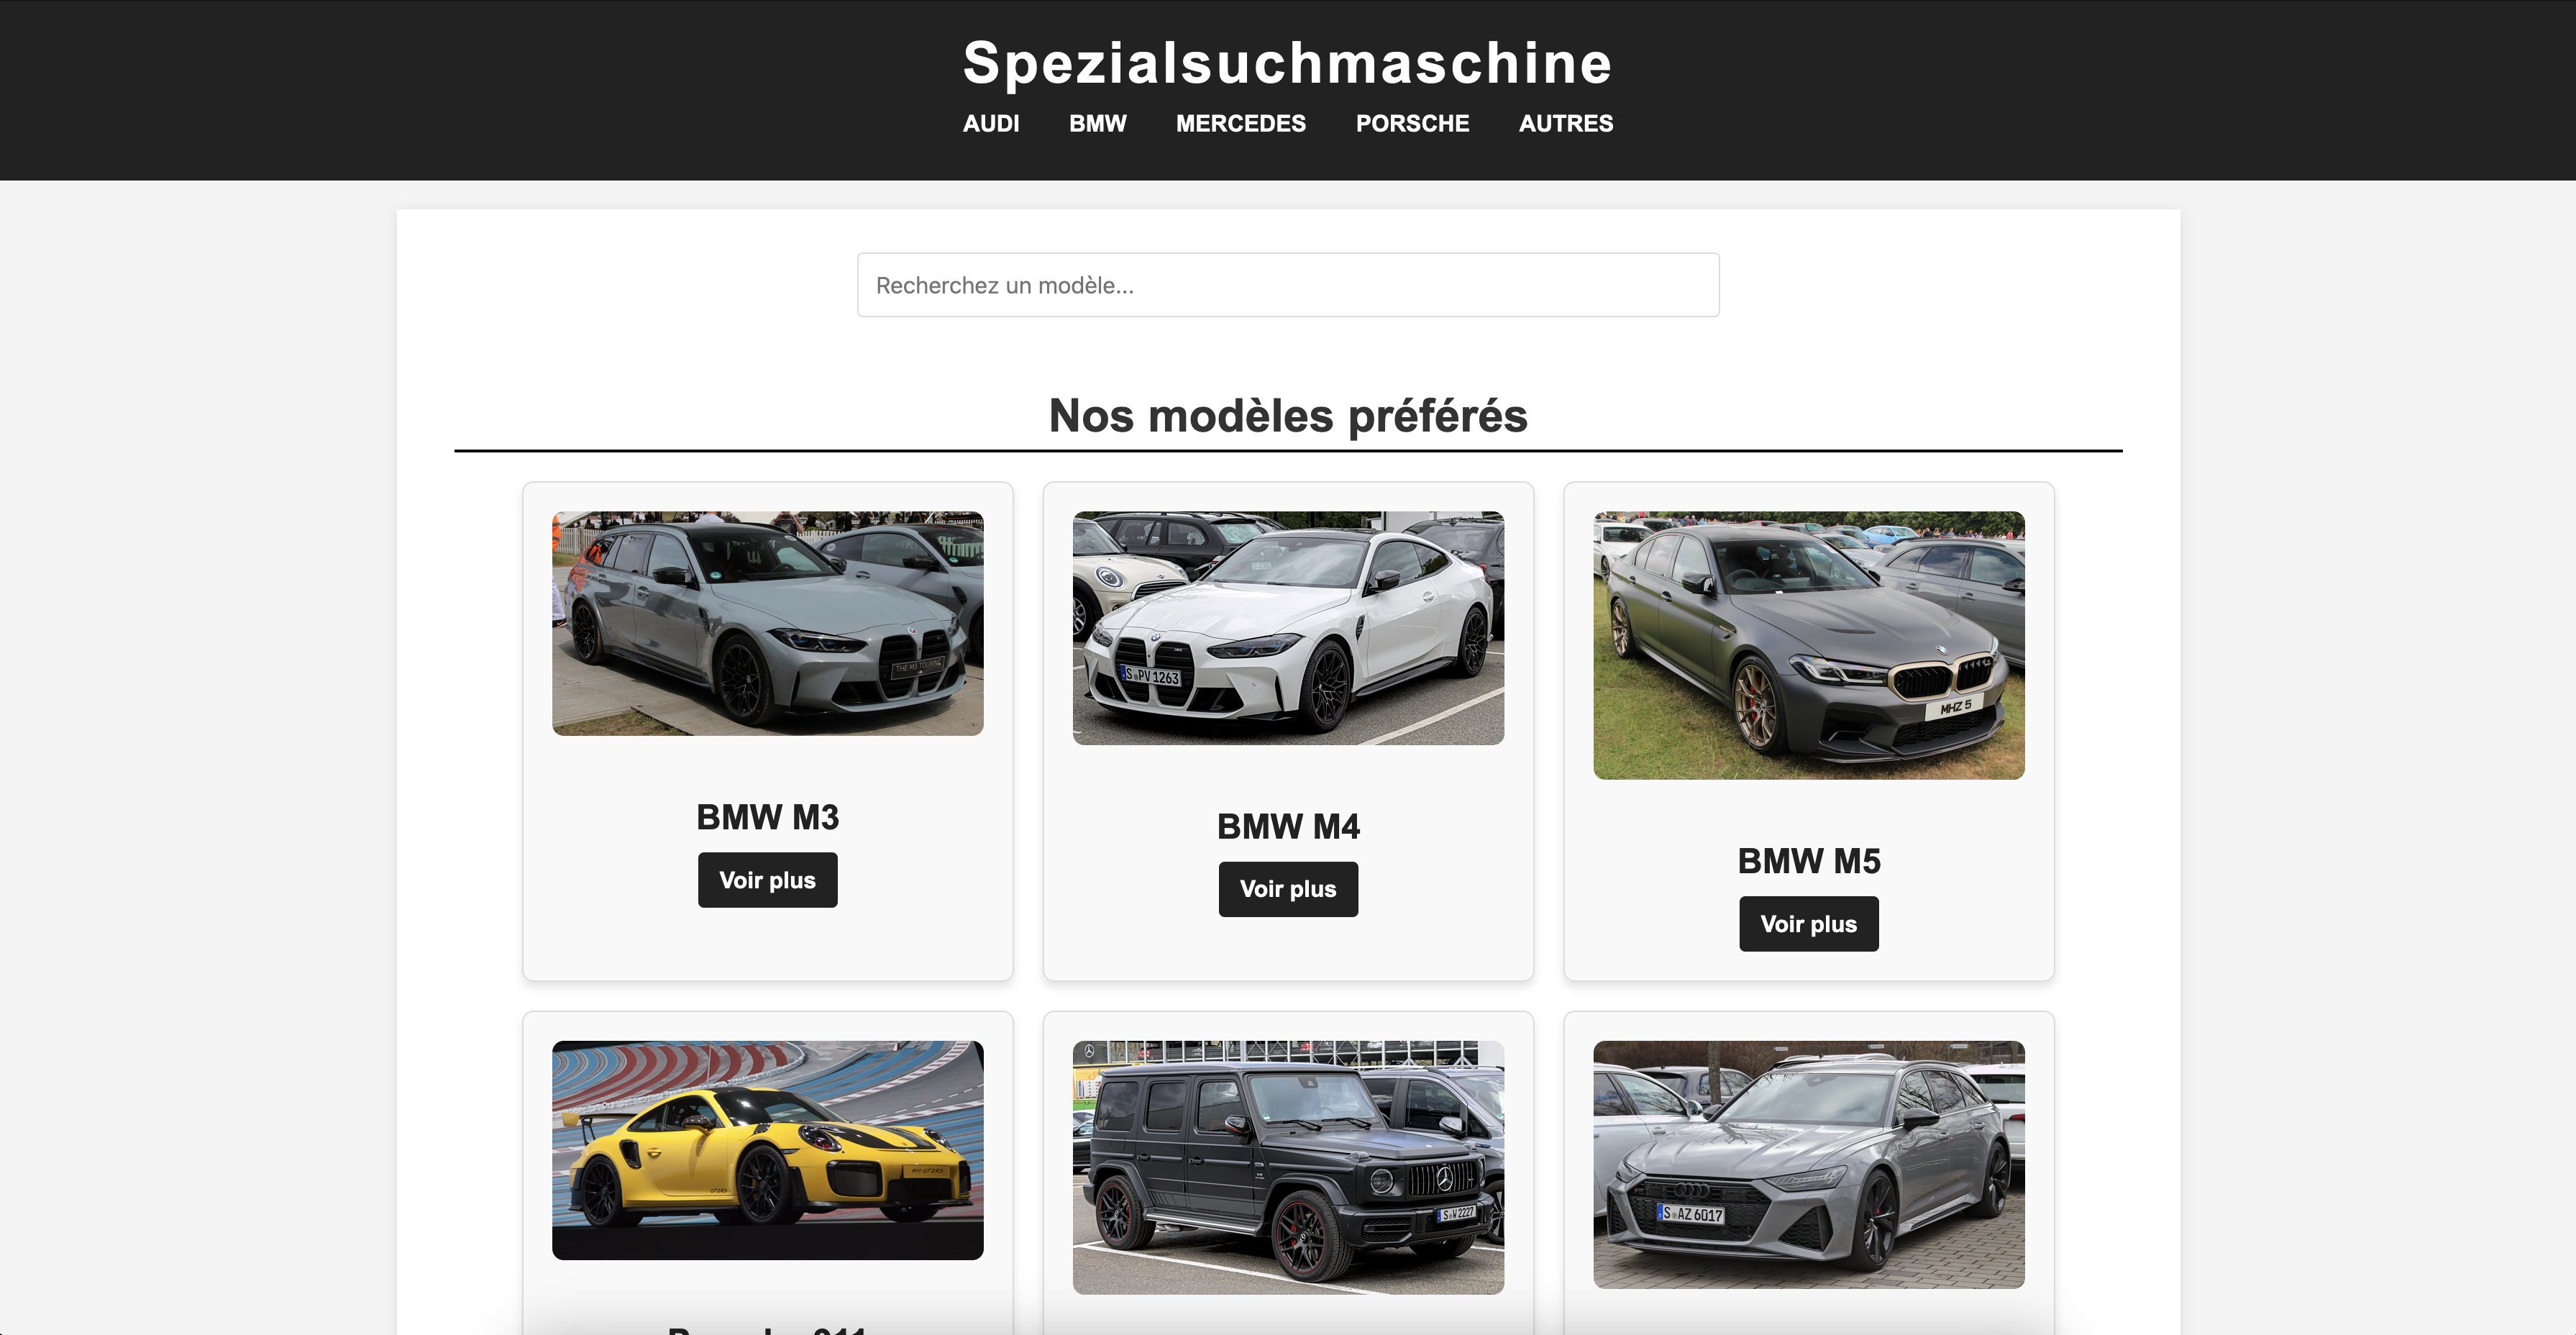
\includegraphics[width=0.8\textwidth]{images/index.png}
\end{frame}

\begin{frame}{Barre de recherche}
\centering
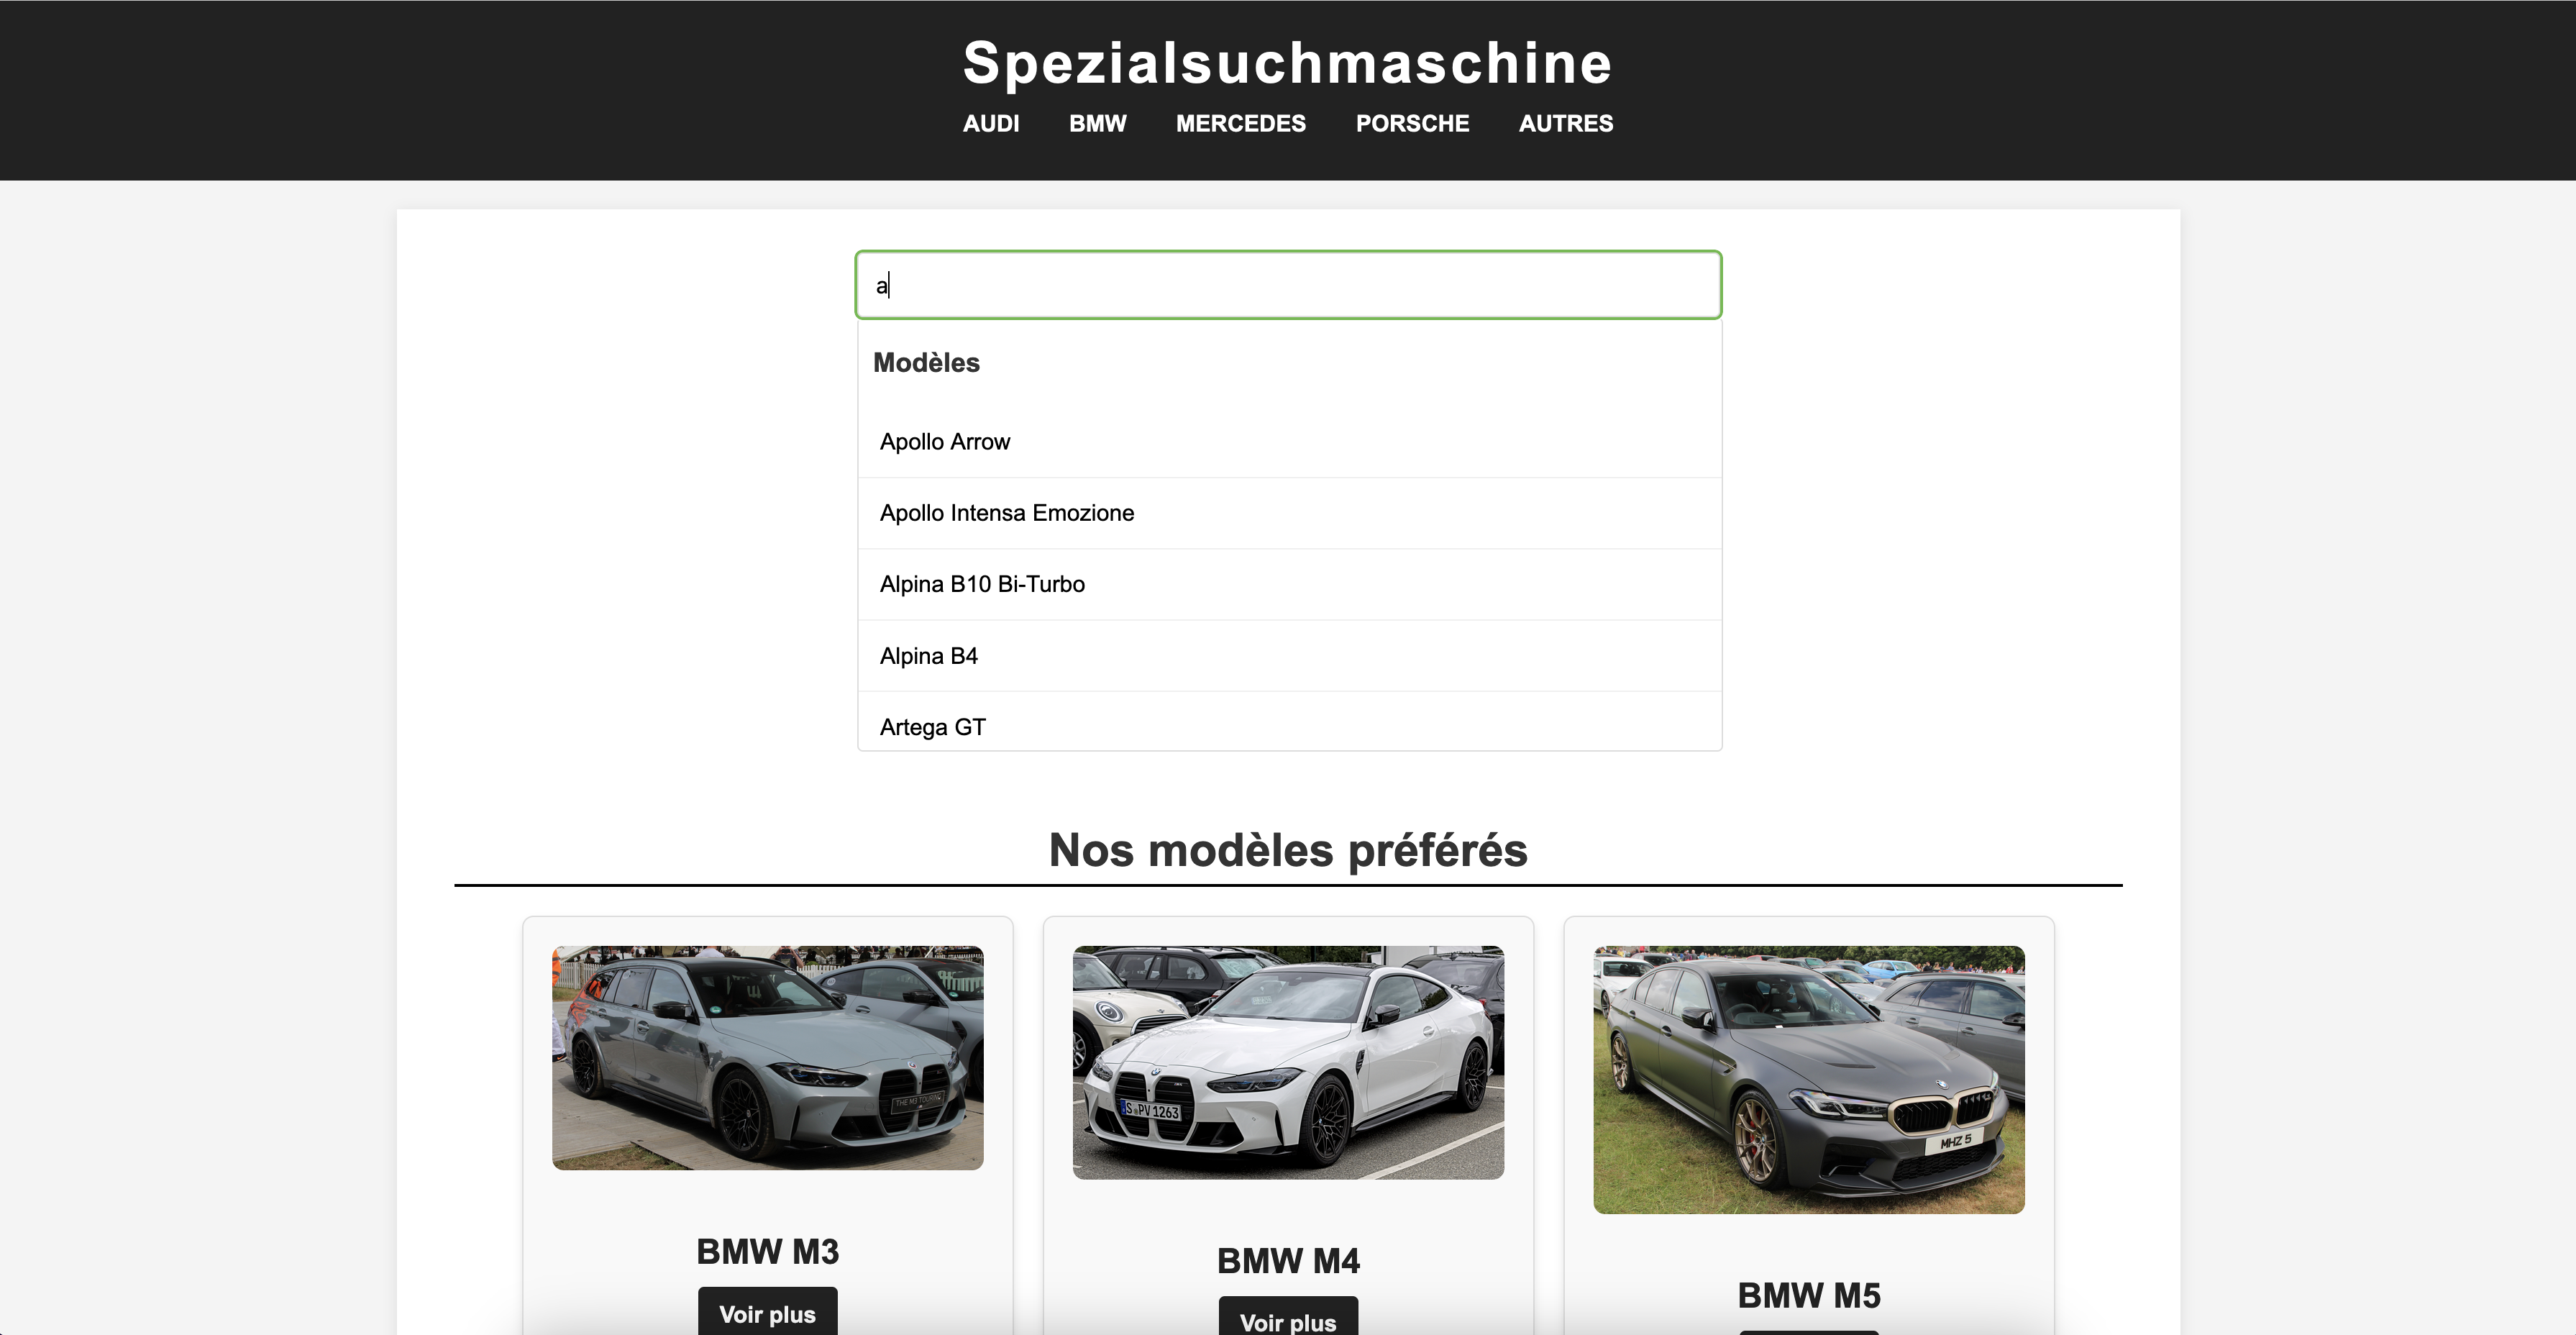
\includegraphics[width=0.8\textwidth]{images/recherche.png}
\end{frame}

\begin{frame}[fragile]{Requête SPARQL}
Rechercher les modèles allemands commencant par "A" :
{\footnotesize
\begin{verbatim}
SELECT DISTINCT ?model ?modelLabel ?manufacturer ?manufacturerLabel
WHERE {
    ?manufacturer dct:subject dbc:Car_manufacturers_of_Germany .

    ?model (dbo:manufacturer|dbp:manufacturer) ?manufacturer .
    ?model rdf:type dbo:Automobile .

    ?model rdfs:label ?modelLabel .
    FILTER(LANG(?modelLabel) = "fr") .
    ?manufacturer rdfs:label ?manufacturerLabel .
    FILTER(LANG(?manufacturerLabel) = "fr") .
    FILTER(REGEX(STR(?modelLabel), "^A", "i")) .
}
LIMIT 5
\end{verbatim}
}
\end{frame}

\begin{frame}[fragile]{Requête SPARQL}
Rechercher les marques automobile allemandes commencant par "A" :  
{\footnotesize
\begin{verbatim}
SELECT DISTINCT ?manufacturer ?manufacturerLabel 
WHERE {
    ?manufacturer dct:subject dbc:Car_manufacturers_of_Germany .
    ?manufacturer rdfs:label ?manufacturerLabel .
    FILTER(LANG(?manufacturerLabel) = "en") .
    FILTER(REGEX(STR(?manufacturerLabel), "^${userInput}", "i")) .
}
ORDER BY ASC(?manufacturerLabel) 
LIMIT 5
\end{verbatim}
}
\end{frame}

\begin{frame}{Affichage des informations d'un modèle}
\centering
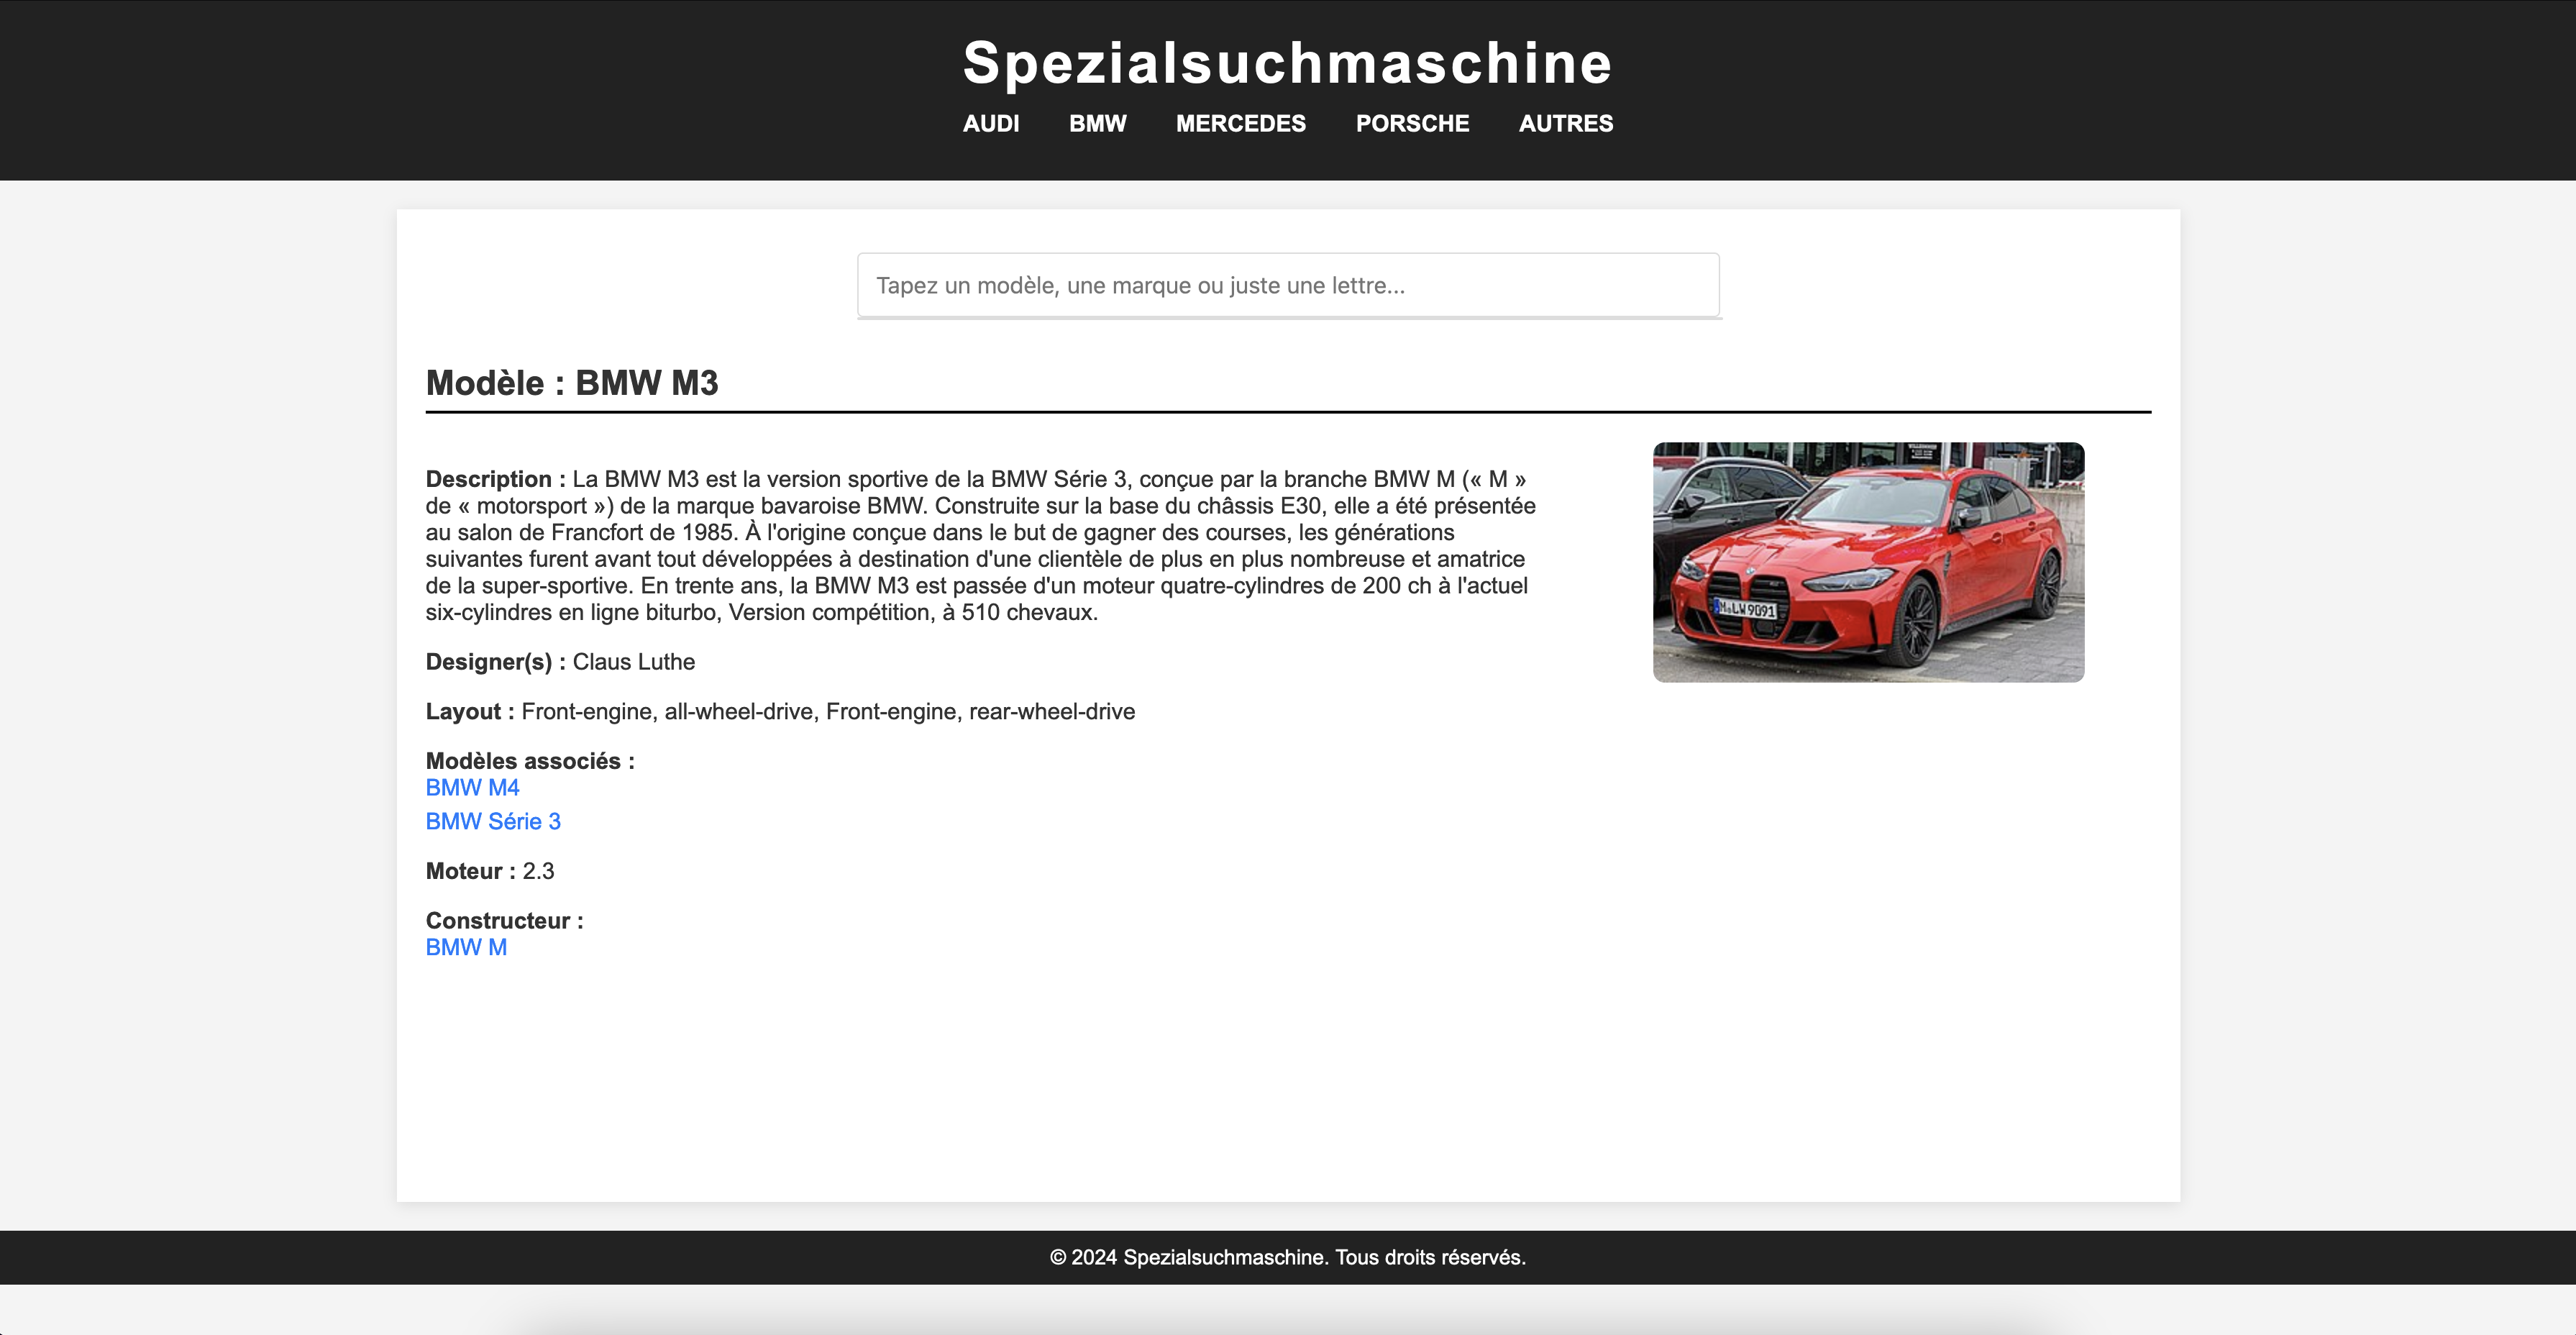
\includegraphics[width=0.8\textwidth]{images/modele.png}
\end{frame}

\begin{frame}[fragile]{Exemple de requête SPARQL}
Obtenir la configuration d'une voiture:
{\footnotesize
\begin{verbatim}
SELECT DISTINCT ?layoutLabel
WHERE {
OPTIONAL {
    <http://dbpedia.org/resource/BMW_M3> dbp:layout ?layout .
    ?layout rdfs:label ?layoutLabel .
    FILTER(LANG(?layoutLabel) = "en") .
}
}
\end{verbatim}
}
\end{frame}

\begin{frame}{Affichage des informations d'une marque}
\begin{itemize}
    \item Recherche de la liste de toutes les  marques de voitures allemandes pour la page principale des marques - requete SPARQL
    \item Récupération des données pour chaque marque, notamment :
    \begin{itemize}
        \item Description, Propriétaire, Chiffre d’affaire, Ville, Date de fondation, Produit, Site Web officiel(lien)
    \end{itemize}
    \item Création dynamique d’une page Web pour chaque marque lors d’une redirection/recherche  vers celle ci - requete SPARQL
\end{itemize}
\end{frame}


\begin{frame}{Affichage des informations d'une marque}
\centering
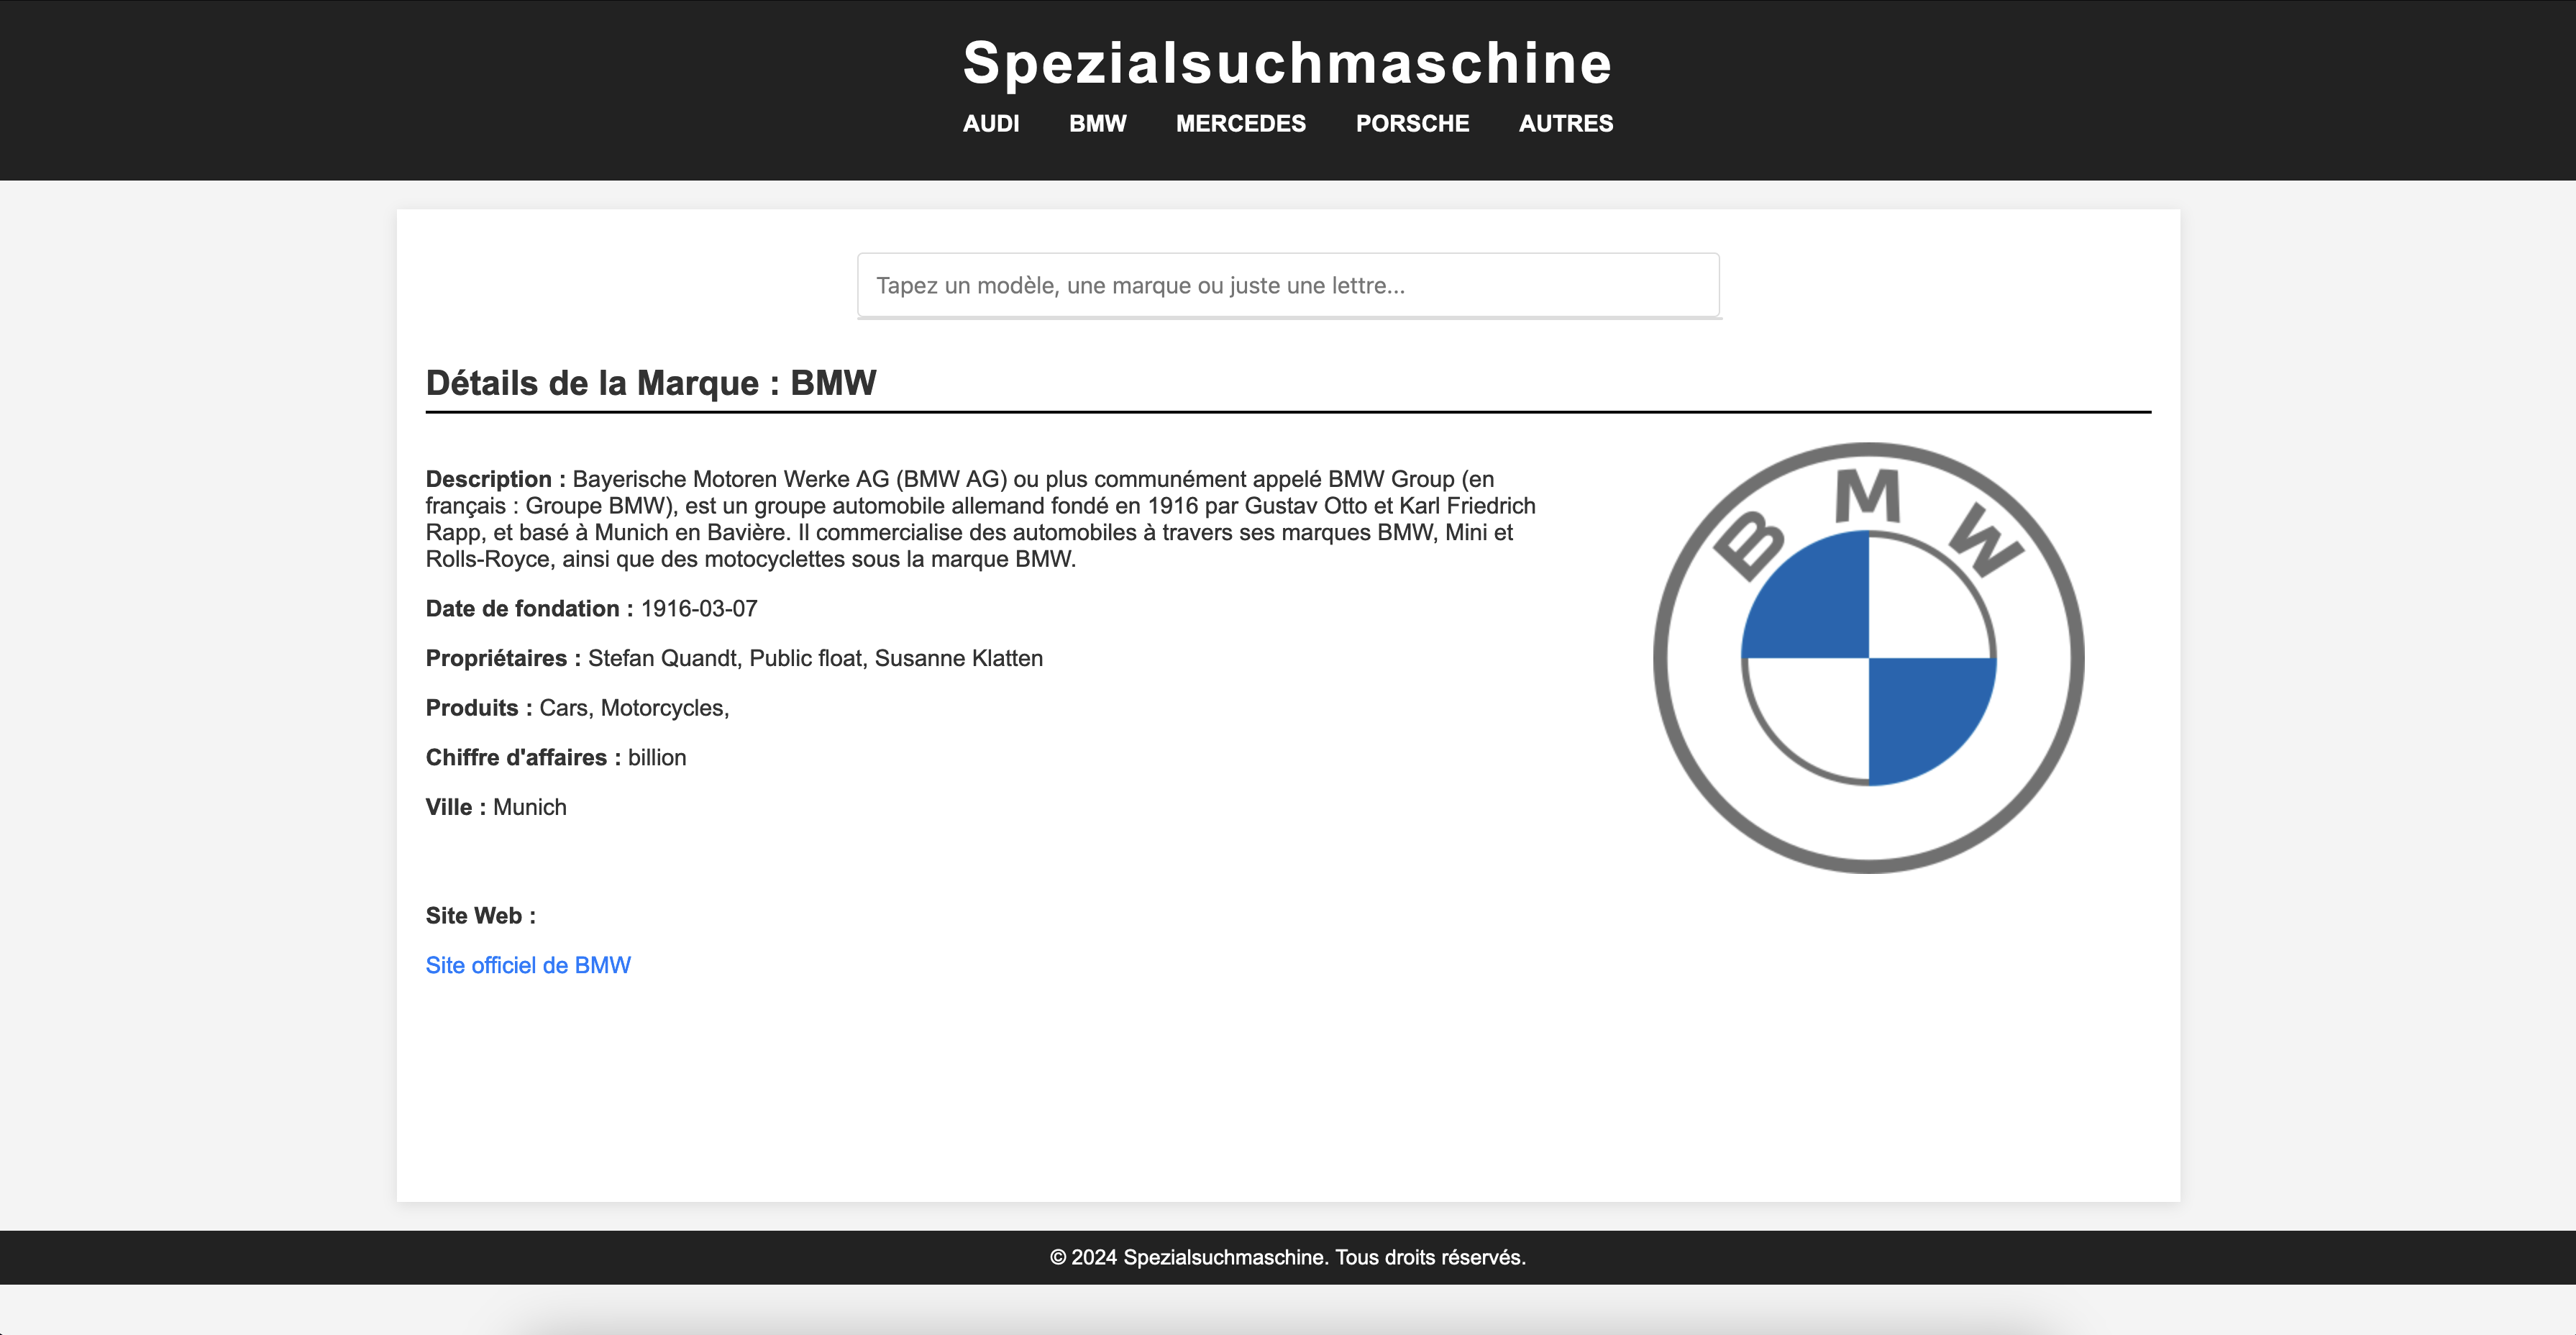
\includegraphics[width=0.8\textwidth]{images/marque.png}
\end{frame}

\begin{frame}[fragile]{Exemple de requête SPARQL}
Obtenir la ville où BMW est implantée:
{\footnotesize
\begin{verbatim}
SELECT DISTINCT ?locationCity ?locationCityName
WHERE {
OPTIONAL {
    <http://dbpedia.org/resource/BMW> dbp:locationCity ?locationCity .
    ?locationCity rdfs:label ?locationCityName .
    FILTER(LANG(?locationCityName) = "en") .
    }
    OPTIONAL {
    <http://dbpedia.org/resource/BMW> dbo:location ?locationCity .
    ?locationCity rdfs:label ?locationCityName .
    FILTER(LANG(?locationCityName) = "en") .
    }
}
\end{verbatim}
}
\end{frame}

\begin{frame}{Affichage des marques automobile allemandes}
\centering
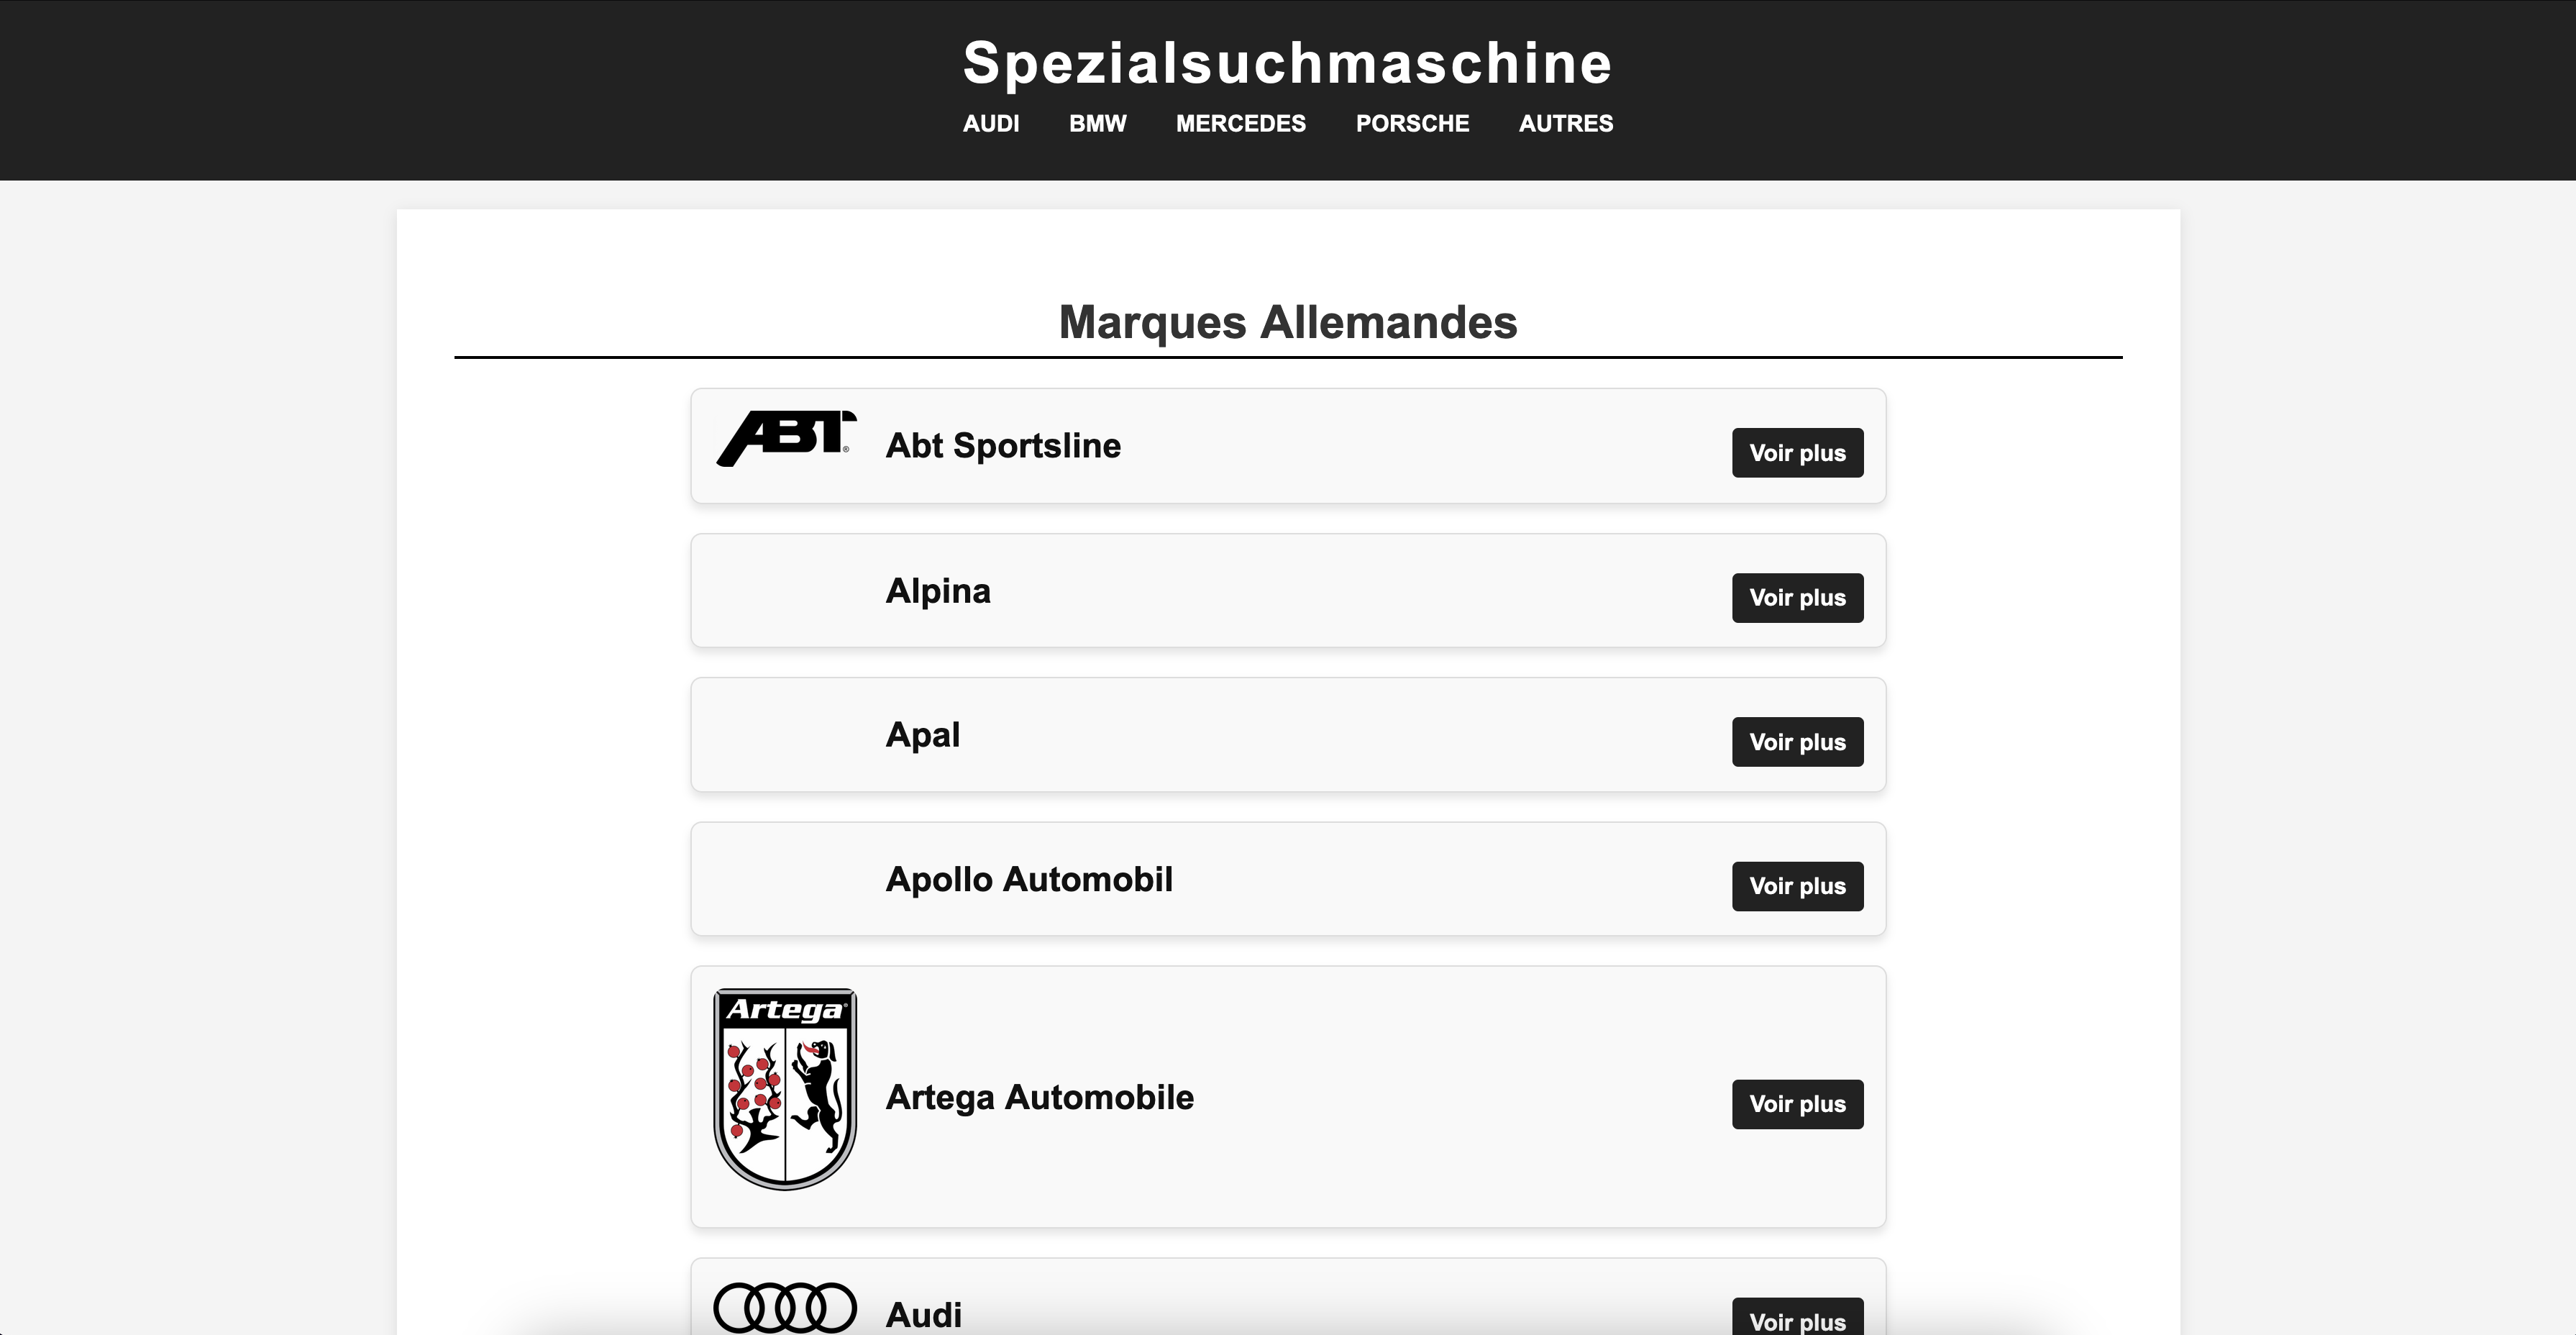
\includegraphics[width=0.8\textwidth]{images/marques.png}
\end{frame}

%------------------------------------------------------------
\section{Technologies utilisées}
\begin{frame}{Technologies utilisées}
\begin{itemize}
    \item \textbf{HTML/CSS} : Structure et mise en forme de l'interface.  
    \item \textbf{JavaScript} : Pour récupérer et afficher les résultats des requêtes SPARQL.  
    \item \textbf{SPARQL} : Requêtes pour extraire des données depuis DBpedia.  
    \item \textbf{DBpedia} : Source principale pour les données liées aux marques automobiles allemandes.  
\end{itemize}
\end{frame}

\begin{frame}[fragile]{Exemple de code HTML}
\begin{center}
\begin{minipage}{0.9\textwidth} % Réduit la largeur à 80% de la page
\begin{lstlisting}[language=HTML, caption=Exemple de requête HTML]
// modele.html
<div id="model-container" class="flex-container">
    <div id="model-details" class="left-column">
        <p>
        <strong>Description :</strong>
        <span id="model-description">Chargement...</span>
        </p>
    </div>
    // reste des informations
</div>
\end{lstlisting}
\end{minipage}
\end{center}
\end{frame}

\begin{frame}[fragile]{Exemple de code JavaScript}
\begin{center}
\begin{minipage}{0.8\textwidth} % Réduit la largeur à 80% de la page
\begin{lstlisting}[language=JavaScript, caption=Exemple de script JavaScript]
// Exemple de fonction JavaScript
async function displayModelInfo() {
    const modelName = getModelNameFromURL();
    const abstractResults = await executeSparqlQuery(
        getModelAbstract(modelName)
    );

    const abstract = getValue(abstractResults, "abstract");

    updateContainer("model-description", abstract);
}
function getModelAbstract(userInput) {
    return `SELECT DISTINCT ?abstract
WHERE {
OPTIONAL {
    <http://dbpedia.org/resource/${userInput}> dbo:abstract ?abstract .
    FILTER(LANG(?abstract) = "fr") .
} 
}`;
}
\end{lstlisting}
\end{minipage}
\end{center}
\end{frame}

%------------------------------------------------------------
\section{Réflexion sur le Web Sémantique}
\begin{frame}{Réflexion sur le Web Sémantique}
\begin{itemize}
    \item Avantages :  
        \begin{itemize}
            \item Accès à des données structurées et interconnectées.  
            \item Utilisation de SPARQL pour des requêtes complexes.  
        \end{itemize}
    \item Inconvénients / Problèmes rencontrés :  
        \begin{itemize}
            \item Dépendance à une source externe (DBpedia).  
            \item Temps de réponse variable et risque d'indisponibilité.  
            \item Syntaxe SPARQL parfois complexe pour des débutants.  
        \end{itemize}
\end{itemize}
\end{frame}

%------------------------------------------------------------
\section{Conclusion}
\begin{frame}{Conclusion}
\begin{itemize}
    \item \textbf{Bilan} : Création réussie d'une application fonctionnelle exploitant le Web Sémantique.  
    \item \textbf{Compétences acquises} :  
        \begin{itemize}
            \item Utilisation de SPARQL pour interroger des bases de données sémantiques.  
            \item Intégration dynamique des résultats avec JavaScript.  
            \item Conception d'une interface ergonomique avec HTML/CSS.  
        \end{itemize}
    \item \textbf{Perspectives} :  
        \begin{itemize}
            \item Ajouter des détails supplémentaires pour chaque marque (images, historique).  
            \item Explorer d'autres sources de données liées au Web Sémantique.  
        \end{itemize}
\end{itemize}
\end{frame}

%------------------------------------------------------------
\section*{Acknowledgement}
\begin{frame}
\textcolor{myNewColorA}{\Huge{\centerline{Merci pour votre attention !}}}
\end{frame}

\end{document}